% GENERATED by scripts/make_figures.py from report/data/report_data.json. Do not edit; regenerate.
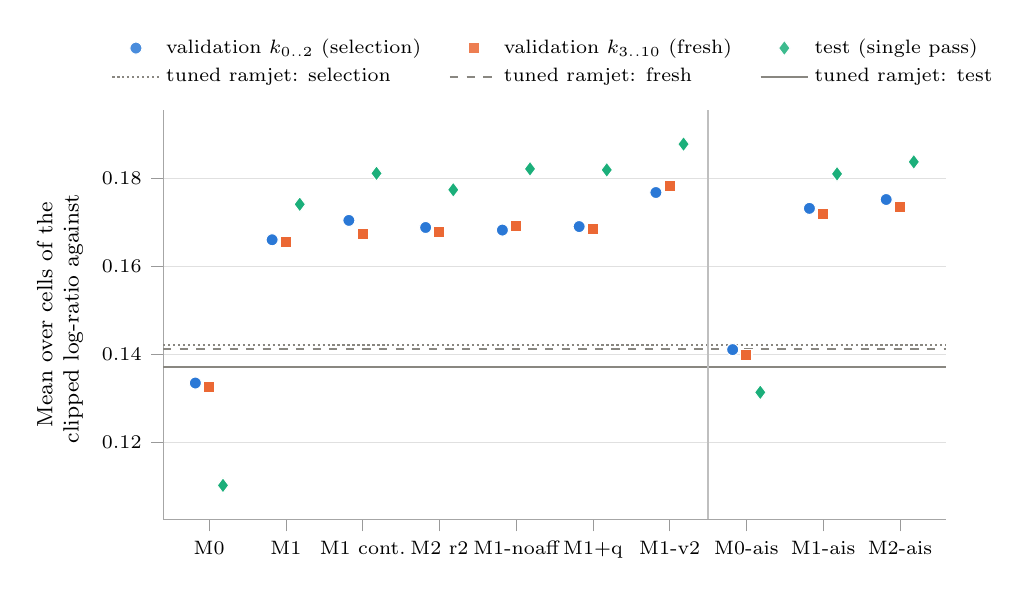
\begin{tikzpicture}
\begin{axis}[
  width=0.82\linewidth, height=5.2cm,
  scale only axis,
  tick label style={font=\scriptsize}, label style={font=\footnotesize, align=center},
  scaled ticks=false, tick label style={/pgf/number format/fixed},
  tick align=outside, tick style={black!40}, axis line style={black!35},
  axis x line*=bottom, axis y line*=left,
  grid style={black!12, line width=0.4pt},
  legend style={font=\scriptsize, draw=none, fill=white, fill opacity=0.85, text opacity=1},
  legend cell align=left,
  xmin=-0.6, xmax=9.6, xtick={0,1,2,3,4,5,6,7,8,9}, xticklabels={{M0},{M1},{M1 cont.},{M2 r2},{M1-noaff},{M1+q},{M1-v2},{M0-ais},{M1-ais},{M2-ais}},
  ymajorgrids, ylabel={Mean over cells of the\\clipped log-ratio against $\piref$},
  legend style={at={(0.5,1.03)}, anchor=south, legend columns=3, /tikz/every even column/.append style={column sep=8pt}},
]
% data: rungs.selection
\addplot[only marks, mark=*, mark size=2.2pt, color={rgb,255:red,42;green,120;blue,214}, mark options={draw=white, line width=0.4pt}] coordinates {(-0.18,0.13342890354099643) (0.8200000000000001,0.16599470141735354) (1.82,0.1704010804209599) (2.82,0.16878966053653194) (3.82,0.16820085589858194) (4.82,0.1690002698298348) (5.82,0.1767435156036474) (6.82,0.14102164778955317) (7.82,0.17313714730249014) (8.82,0.1751499238515255)};
\addlegendentry{validation $k_{0..2}$ (selection)}
% data: rungs.fresh
\addplot[only marks, mark=square*, mark size=2pt, color={rgb,255:red,235;green,104;blue,52}, mark options={draw=white, line width=0.4pt}] coordinates {(0.0,0.13262963505096179) (1.0,0.16556456087816657) (2.0,0.167237480661827) (3.0,0.16774290438003298) (4.0,0.1692366009703472) (5.0,0.16836845964916694) (6.0,0.17830748263632787) (7.0,0.13970245464408904) (8.0,0.17180490670878812) (9.0,0.17350843809790512)};
\addlegendentry{validation $k_{3..10}$ (fresh)}
% data: rungs.test
\addplot[only marks, mark=diamond*, mark size=2.8pt, color={rgb,255:red,27;green,175;blue,122}, mark options={draw=white, line width=0.4pt}] coordinates {(0.18,0.11016641308341514) (1.18,0.17406140813739945) (2.18,0.18110069617862282) (3.18,0.17736484274621056) (4.18,0.18211393631847803) (5.18,0.18187320385634786) (6.18,0.18774355882517585) (7.18,0.13130833932846517) (8.18,0.18097536262899377) (9.18,0.18370126112559385)};
\addlegendentry{test (single pass)}
% data: ramjet.selection
\addplot[color={rgb,255:red,137;green,135;blue,129}, densely dotted, line width=0.8pt, no marks] coordinates {(-0.6,0.14201773497049403) (9.6,0.14201773497049403)};
\addlegendentry{tuned \policy{ramjet}: selection}
% data: ramjet.fresh
\addplot[color={rgb,255:red,137;green,135;blue,129}, dashed, line width=0.8pt, no marks] coordinates {(-0.6,0.1411348331803814) (9.6,0.1411348331803814)};
\addlegendentry{tuned \policy{ramjet}: fresh}
% data: ramjet.test
\addplot[color={rgb,255:red,137;green,135;blue,129}, solid, line width=0.8pt, no marks] coordinates {(-0.6,0.13715999535272497) (9.6,0.13715999535272497)};
\addlegendentry{tuned \policy{ramjet}: test}
\draw[black!25, line width=0.8pt] ({axis cs:6.5,0} |- {rel axis cs:0,0}) -- ({axis cs:6.5,0} |- {rel axis cs:0,1});
\end{axis}
\end{tikzpicture}
